\documentclass{standalone}
\usepackage{tikz}
\usepackage[dvipsnames]{xcolor}
\usepackage{amsthm, amsmath, mathtools, amssymb, physics} % for math and physics commands and symbols.

\begin{document}
  
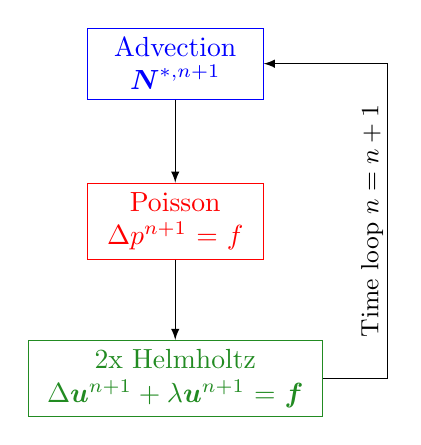
\begin{tikzpicture}
    \node[draw,align=center,color=blue] (Adv) [text width=2cm] at (0,0) {Advection $\boldsymbol{N}^{*,n+1}$};
    \node[draw,align=center,color=red] (P) [text width=2cm] at (0,-2) {Poisson $\Delta p^{n+1} = f$};
    \node[draw,align=center,color=ForestGreen] (H) [text width=3.5cm] at (0,-4) {2x Helmholtz $\Delta \boldsymbol{u}^{n+1} + \lambda \boldsymbol{u}^{n+1} = \boldsymbol{f}$};
    \node[rotate=90] (Tl) at (2.5,-2) {\small Time loop $n=n+1$};

    % Arrows
    \draw[-latex] (Adv) edge (P) (P) edge (H) (H) -- (2.7,-4) -- (2.7,0) -- (Adv);
\end{tikzpicture}

\end{document}
